\documentclass{article}
\usepackage{tikz}
\usepackage{pgfplots}
\usepackage{xcolor}
\usepackage{svg}
\usepackage{amsmath}
\usepackage{array}
\usepackage[skins]{tcolorbox}
\usepackage[version=4]{mhchem}
\usepackage[a4paper, total={6in, 9in}]{geometry}
\usepackage{fourier}
\usepackage{xymtex}
\usepackage{textcomp}
\usepackage{eurosym}
\usepackage{caption}
\usepackage{longtable}
\usepackage{float}
\usepackage{attachfile}
\usepackage{multirow}

\captionsetup[table]{name=\textit{Tabella}}
\pagenumbering{gobble}

\title{Relazione di laboratorio - pendolo di Kater}
\author{Federico Cesari}
\date{7 gennaio 2024}




\begin{document}
	\begin{titlepage}
	\begin{center}
		\vspace*{1cm}
		
		\textbf{\LARGE Relazione di laboratorio - Pendolo semplice}
		
		\vspace{0.3cm}
		\large \textit{Misura del periodo di un pendolo semplice} \\
		
		\vspace{0.5cm}
		\Large Federico Cesari \\
		
		\small 1096759 
		\vspace{0.2cm}
		
		\small Gruppo 5
		
		
		\vspace{3cm}
		\begin{center}
			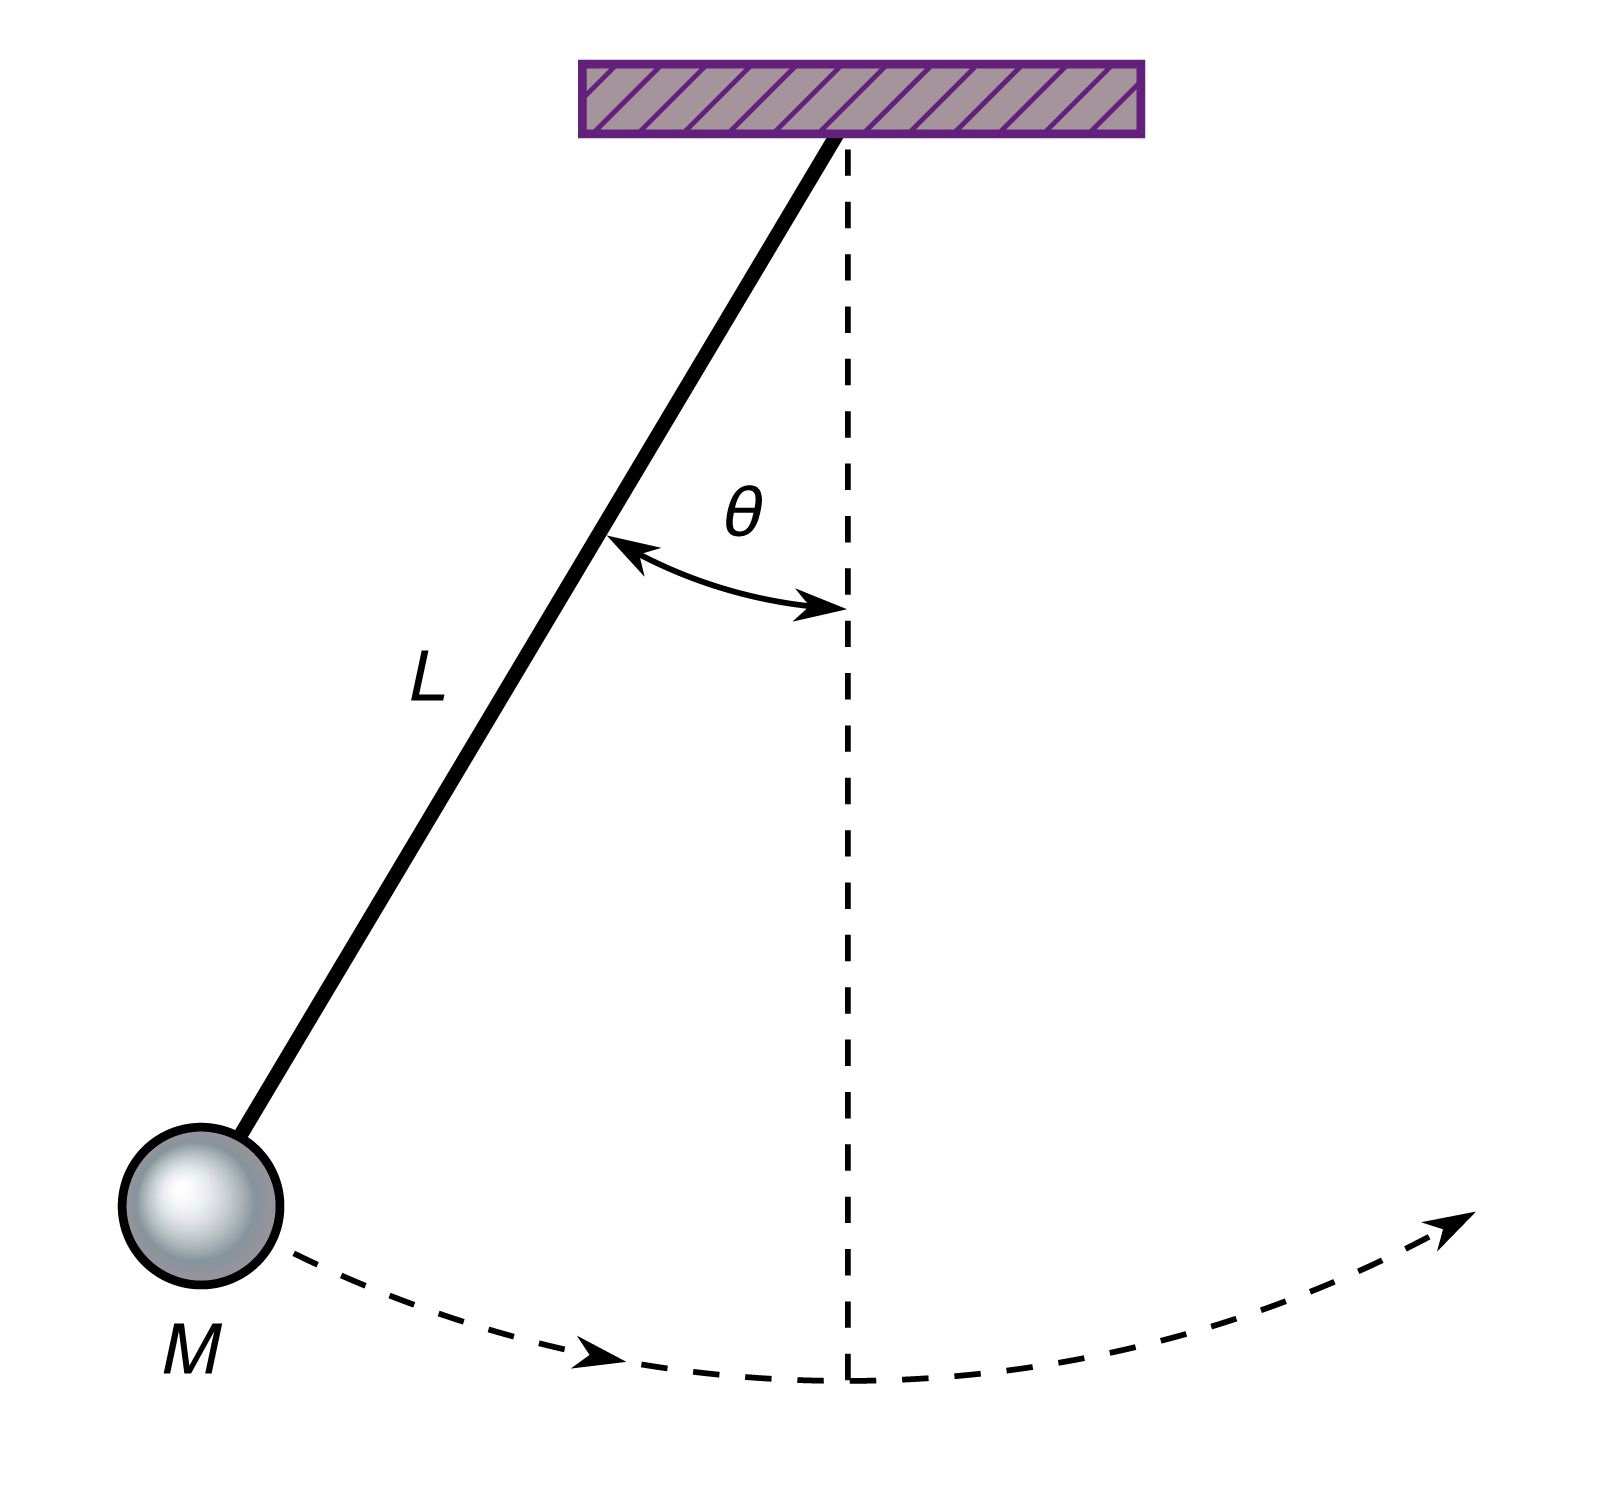
\includegraphics[scale=0.1]{IMG_0200.jpeg}	
		\end{center}
		
		
		
		\vfill
		
		
		
		corso A\\
		Università degli studi di Torino, Torino\\
		4 aprile 2024\\
		
		
	\end{center}
\end{titlepage}

	
	\section{Scopo dell'esperienza}
	L'esperienza di laboratorio ha lo scopo di determinare il periodo di oscillazione di un pendolo fisico in presenza di errori casuali (ed eventualmente di errori sistematici) e verificare che i valori misurati per mezzo di un cronometro siano accurati o meno rispetto alle misure effettuate da una fotocellula. 
	
	\vspace{0.5cm}
	\begin{table}[H]
		\centering
		\renewcommand{\arraystretch}{1.5}
		\begin{tabular}{lr}
			 & \textit{sensibilità}\\
			 \hline
			Cronometro $\quad$                	& $0.01s$    \\
			Fotocellula  $\quad$                & $0.001s$    \\
		\end{tabular}
		\renewcommand{\arraystretch}{1}
		\captionof*{table}{\textbf{Strumenti}}
	\end{table}
	\vspace{0.5cm}
	
	Tramite una registrazione del pendolo, con l'aiuto di un cronometro digitale ne ho misurato il periodo di oscillazione registrando cento misure su un foglio di calcolo. 
	
	
	

	\section{Prima osservazione dati}
	
	Dalle cento misure ho ricavato i valori nella \textit{Tabella 1}. Il più piccolo valore rilevato ($1.59s$) e il più grande ($2.31s$) decido di escluderli secondo il criterio di rigetto a $3\sigma_{x}$.
	
	\paragraph{Criterio di rigetto a $\mathbf{3\sigma}$}
	Il test permette di identificare quei valori che non appartengono alla popolazione che si sta analizzando. So infatti che le mie misure hanno il $99.7 \%$ di probabilità di ricadere nell'intervallo $(\bar{x}  - 3\sigma_{x} , \bar{x} + 3\sigma_{x})$, dove $\bar{x}$ è la media della popolazione e $\sigma_{x}$ è la deviazione standard. La probabilità di osservare una misura al di fuori di questo intervallo risulterebbe essere di circa lo $0.3\%$, che su 100 misure è come se non  se ne osservasse nessuna. Posso quindi affermare che valori osservati oltre $3 \sigma_{x}$ appartengono a un'altra popolazione e, di conseguenza, che è lecito rigettarli. 
	
	Successivamente al rigetto, con i $98$ dati rimanenti ricavo i nuovi valori riportati nella \textit{Tabella 2}.
	
	\vspace{0.8cm}
	\begin{minipage}[c]{0.45\textwidth}
		\centering
		\begin{tabular}{llrl}
			Media                       & $\bar{x}$             & $1.95$        & $s$       \\
			Varianza                    & $\sigma_{x}^2$          & $0.0092$     & $s^2$  \\
			Dev. std                    & $\sigma_{x}$              & $0.096$      & $s$   \\
			Dev. std (della media)      & $\sigma_{\bar{x}}$    & $0.0096$     & $s$    \\
			Mediana                     & $\mu_e$               & $1.95$        &  $s$      \\
			Moda                        & $v_0$                 & $2.00$        & $s$
		\end{tabular}
		\captionof{table}{\textit{100 misure}}
	\end{minipage}
	\begin{minipage}[c]{0.5\textwidth}
		\centering
		\begin{tabular}{llrl}
			Media                       & $\bar{x}$             & $1.95$        & $s$       \\
			Varianza                    & $\sigma_{x}^2$          & $0.0068$     & $s^2$  \\
			Dev. std                    & $\sigma_{x}$              & $0.082$      & $s$   \\
			Dev. std (della media)      & $\sigma_{\bar{x}}$    & $0.0083$     & $s$    \\
			Mediana                     & $\mu_e$               & $1.95$        &  $s$      \\
			Moda                        & $v_0$                 & $2.00$        & $s$
		\end{tabular}
		\captionof{table}{\textit{98 misure}}
	\end{minipage}
	\vspace{0.8cm}
	
	\noindent
	Confrontando i valori nelle due tabelle si notano una sensibile diminuzione della varianza ($-26 \%$) e una variazione della deviazione standard e della deviazione standard della media (entrambe circa $-13 \%$). Variazioni prevedibili vista l'esclusione di valori molto distanti dalla media della popolazione. \\
	
	\noindent
	Procedo accorpando i dati in 13 classi ognuna "larga" $0.04s$.
	
	\vspace{0.8cm}
	\begin{table}[H]
		\centering
		\begin{tabular}{llrl}
			Media                       & $\bar{x}$             & $1.95$        & $s$       \\
			Varianza                    & $\sigma_{x}^2$          & $0.0067$     & $s^2$  \\
			Dev. std                    & $\sigma_{x}$              & $0.082$      & $s$   \\
			Dev. std (della media)      & $\sigma_{\bar{x}}$    & $0.0083$     & $s$    
		\end{tabular}
		\captionof{table}{\textit{Dati accorpati}}
	\end{table}
	\vspace{0.5cm}
	
	\noindent
	I dati accorpati producono valori pressoché identici a quelli rilevati post rigetto a $3\sigma_{x}$. \\
	
	
	\noindent
	\paragraph{Errore sulla stima} La sensibilità del cronometro da me utilizzato è $0.01s$, ciò significa che lo strumento non può distinguere o rilevare variazioni inferiori a tale valore. La deviazione standard calcolata mi dice invece che le mie misure hanno una dispersione naturale attorno al valor medio uguale a $0.008s$, quindi contenuta nei limiti di precisione dello strumento. Poiché l'errore "naturale", dettato unicamente dal caso, risulta non misurabile dal cronometro scelgo la sensibilità $0.01s$ come errore sulla stima.  \\
	
	\paragraph{Migliore stima} Dopo aver escluso i dati appartenenti a un'altra popolazione e raggruppato i dati, la mia migliore stima del  periodo di oscillazione del pendolo è:
	\[
	\mathbf{1.95s \quad \pm \quad 0.01 s}
	\]
	
	
	
	
	
	\newpage
	\section{Test $\chi ^2$ di adattamento}
	Poiché mi aspetto che le mie misure fluttuino attorno al mio valor medio e che siano soggette a soli errori casuali, è ragionevole pensare che esse siano governate da una distribuzione limite di tipo gaussiano centrata nel valore corrispondente alla mia migliore stima $\bar{x}$. Eventuali errori sistematici traslerebbero la curva lungo l'asse orizzontale allontanando $\bar{x}$ dal valore che considero vero $\mu$ calcolato dalla fotocellula. \\ 
	
	\noindent
	Il test del $\chi ^2$ ha proprio lo scopo di verificare che la nostra distribuzione sia consistente con l'ipotesi che le misure siano governate da una certa distribuzione limite.
	
	\vspace{0.6cm}
	\begin{center}
	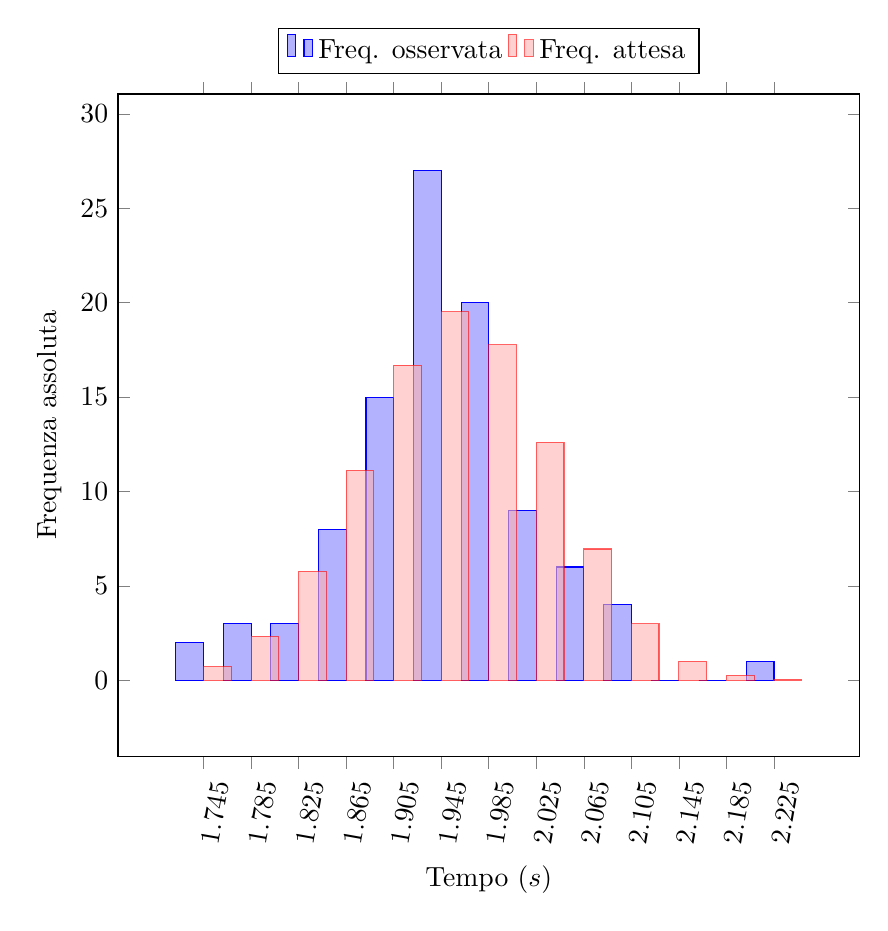
\begin{tikzpicture}
		\pgfplotsset{compat = 1.3}
		\begin{axis}[
			width=11cm, 
			height=10cm,
			ylabel=Frequenza assoluta,
			xlabel=Tempo $(s)$,
			enlargelimits=0.15,
			legend style={at={(0.5,1.1)},	anchor=north,legend columns=-1},
			ybar=0pt,% configures `bar shift'
			bar width=10pt,
			xtick={1.745,
				1.785,
				1.825,
				1.865,
				1.905,
				1.945,
				1.985,
				2.025,
				2.065,
				2.105,
				2.145,
				2.185,
				2.225},
			xticklabels={1.745, 1.785, 1.825, 1.865, 1.905, 1.945, 1.985, 2.025, 2.065, 2.105, 2.145, 2.185, 2.225},
			xticklabel style={rotate=80, anchor=north east}
			]
			\addplot+[opacity=1] 
			coordinates {
			(1.745,2)
			(1.785,3)
			(1.825,3)
			(1.865,8)
			(1.905,15)
			(1.945,27)
			(1.985,20)
			(2.025,9)
			(2.065,6)
			(2.105,4)
			(2.145,0)
			(2.185,0)
			(2.225,1)};
			\addplot+[opacity=0.6]
			coordinates {
			(1.745,0.733)
			(1.785,2.330)
			(1.825,5.767)
			(1.865,11.116)
			(1.905,16.688)
			(1.945,19.510)
			(1.985,17.764)
			(2.025,12.597)
			(2.065,6.957)
			(2.105,2.992)
			(2.145,1.002)
			(2.185,0.261)
			(2.225,0.053)
			};
			\legend{Freq. osservata,Freq. attesa}
		\end{axis}
	\end{tikzpicture}
	\end{center}
	\vspace{0.2cm}
	
	\paragraph{Ipotesi nulla (H$_{0}$)} La distribuzione teorica di Gauss si adatta alla distribuzione delle mie misure. 
	\paragraph{Ipotesi contraria (H$_{1}$)} La distribuzione teorica di Gauss non si adatta alla distribuzione delle mie misure. 
	\noindent
	Scelgo un livello di significatività del $5\%$ e procedo calcolando il valore di $\chi^2$ e il numero di gradi di libertà. Con questi due dati ricavo dalle tabelle di distribuzione il valore del mio $\chi^2$ critico. 
	\vspace{0.4cm}
	\begin{table}[H]
		\centering
		\begin{tabular}{lr}
			Livello di significatività 		& $ \quad 5\%$  \\
			Valore di $\chi ^2$             & $\quad 6.39$       \\
			Numero di gradi di libertà      & $\quad (7-2-1) = 4$         \\   
			Valore di $\chi ^2$ critico     & $\quad 9.48$
		\end{tabular}
		\captionof{table}{\textit{Dati per il test $\chi^2$ di adattamento}}
	\end{table}
	 
	\paragraph{Conclusione del test} Poiché $\chi^2 < \chi^2_{\text{critico}}$ , la  discrepanza tra le frequenze osservate e quelle attese risulta essere accettabile nei livelli di significatività scelti, quindi il risultato del test è in linea con le mie aspettative: la distribuzione di Gauss si adatta a quella delle mie misure. Dico quindi che \colorbox{green}{\textbf{accetto}} l'ipotesi $\text{H}_{0}$ con un livello di significatività del $5\%$. 
	
	Nonostante questo il valore di $\chi^2$ risulta essere confrontabile con quello di $\chi^2_{\text{critico}}$, quindi, seppur rientri nei limiti scelti a priori dal livello di significatività, è da considerare che la discrepanza tra frequenze osservate e attese non sia trascurabile e, anzi, sia quasi al limite di tolleranza.
	
	
	\vspace{1cm}
	\section{Test di Gauss}
	Per verificare che il valor medio da me calcolato non si discosti significativamente dal valore misurato dalla fotocellula si utilizzerà il test Z, o test di Gauss. Riporto in ordine la mia stima del periodo e quella misurata dalla fotocellula:
	\[
	\bar{x} = 1.95s \pm 0.01 s
	\]
	\[
	\mu = 1.957s \pm 0.001 s
	\]

	Il test di Gauss ci permette di calcolare la probabilità di osservare medie che distano in valore assoluto più di quanto dista il mio $\bar{x}$ dal valore vero $\mu$ solo per l'influenza di fluttuazioni statistiche. Quindi a seguito del test possiamo capire se i nostri dati producono medie consistenti con il valore vero.\\
	
		\paragraph{Variabile standardizzata $\mathbf{z}$} Per capire il funzionamento del test di Gauss è necessario capire cosa sia la variabile standardizzata $z$. Per prima cosa trovo quanto dista la mia migliore stima del periodo del pendolo dal valore misurato dalla fotocellula in  unità della deviazione standard e lo assegno alla variabile $|z_{\text{oss}}|$:
	\[
	|z_{\text{oss}}| = \frac{\bar{x} - \mu}{\sigma_{\bar{x}}}
	\]
	Mi chiedo quindi quale sia la probabilità di ottenere una discrepanza maggiore del mio $|z_{\text{oss}}|$, ovvero mi chiedo quale sia la probabilità di ricadere nelle code della curva.
	
	Per fare ciò ci è comodo cambiare variabile nella funzione così da ottenere una curva centrata in zero. Definisco una nuova variabile $z$:
	\[
	z = \frac{x-\mu}{\sigma_{\bar{x}}} \qquad \to \qquad \frac{1}{\sqrt{2\pi}} \int_{-t}^{t}e^{-\frac{-z^2}{2}} \,dz
	\]
	
	Questa nuova espressione della curva gaussiana nella variabile standardizzata $z$ è centrata in $0$ ($\mu_z =0$) e ha deviazione standard = 1 ($\sigma_{z} = 1$).
	
	\vspace{0.5cm}
	\begin{center}
		\begin{minipage}[l]{0.45\textwidth}
			\begin{tikzpicture}
				\begin{axis}[
					axis lines = middle,
					xlabel = \( x \),
					ylabel = \( f(x) \),
					ymin = 0,
					ymax = 1.2,
					xmin = -1,
					xmax = 5,
					xtick = {-1,0,1,2,3,4,5},
					xticklabels = { , , \(-\sigma\),,\(\sigma\), ,},
					yticklabel=\empty,
					domain = -1:5,
					samples = 100,
					smooth,
					every axis plot post/.append style={mark=none}
					]
					
					\addplot[blue, thick] {exp(-(x-2)^2)};
				\end{axis}
			\end{tikzpicture}	
		\end{minipage}
		\hspace{0.5cm}
		\begin{minipage}[r]{0.45\textwidth}
			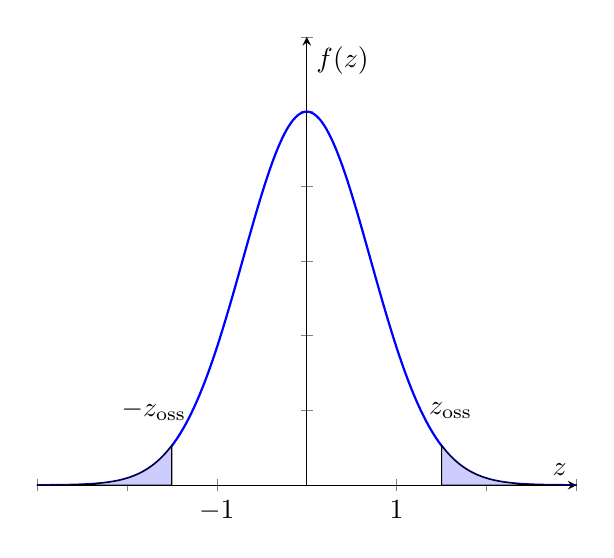
\begin{tikzpicture}
				\begin{axis}[
					axis lines = middle,
					xlabel = \( z \),
					ylabel = \( f(z) \),
					ymin = 0,
					ymax = 1.2,
					xmin = -3,
					xmax = 3,
					xtick = {-3,-2,-1,0,1,2,3},
					xticklabels = { , , \(-1\), 0 ,\(1\), ,},
					yticklabel=\empty,
					domain = -3:3,
					samples = 100,
					smooth,
					every axis plot post/.append style={mark=none}
					]
					
					\addplot[blue, thick] {exp(-x^2)};
					\addplot[fill=blue!20, domain=-3:-1.5] {exp(-x^2)} \closedcycle;
					\addplot[fill=blue!20, domain=1.5:3] {exp(-x^2)} \closedcycle;
					
					\node[] at (axis cs: -1.7, 0.2) {\( -z_{\text{oss}} \)};
					\node[] at (axis cs: 1.6, 0.2) {\( z_{\text{oss}} \)};
					
				\end{axis}
			\end{tikzpicture}	
		\end{minipage}
	\end{center}
	
	
	\noindent
	Il valore di $z_{\text{oss}}$ rappresenta la distanza tra la mia migliore stima $\bar{x}$ e il valore vero $\mu$ in unità di deviazione standard. La probabilità di avere uno $z > z_{\text{oss}}$, quindi l'area nelle code della gaussiana, è descritta dal \textit{p-value}; più il p-value è piccolo, minore è la probabilità che \textit{solo per caso} si osservi una discrepanza maggiore di quella osservata. Se quest'ultima probabilità è bassa significa che la mia discrepanza è già significativamente elevata e che quindi la mia migliore stima si discosta di parecchio dal valore vero.
	(\textit{Il valore minimo accettabile di p-value è deciso a priori ed è detto livello di significatività $\alpha$}).
	
	\paragraph{Ipotesi nulla H$_{0}$} La mia migliore stima del periodo è compatibile con il valore misurato dalla fotocellula $\mu$ nei livelli di significatività scelti	
	\paragraph{Ipotesi contraria H$_{1}$} La mia miglior stima non risulta compatibile con $\mu$ nei livelli di significatività scelti.
	\[
	\mu = 1.957s \pm 0.001 s
	\]
	\begin{table}[H]
		\centering
		\begin{tabular}{lr}
			Livello di significatività $\alpha$		& $ \quad 5\%$  \\
			Valore di $z$ critico     & $\quad 1.96$ \\
			Valore di $|z_{\text{oss}}|$      & $\quad 0.88$ \\
			p-value     & $\quad 0.38$
		\end{tabular}
	\end{table}



	\paragraph{Conclusione}\label{para}  Il p-value è superiore al livello di significatività $\alpha$, quindi \colorbox{green}{\textbf{accetto}} l'ipotesi nulla $H_{0}$ e concludo affermando che la mia stima è compatibile con il valore vero con un livello di significatività del $5\%$. Accettando l'ipotesi nulla posso dire che le mie misure hanno una variabilità dettata unicamente da fluttuazioni statistiche e di conseguenza eventuali  errori sistematici risultano essere trascurabili.
	
	\subsection{Commenti}
	\begin{itemize}
		\item \textit{L'analisi degli errori suggerisce come migliorare la procedura di misurazione o gli strumenti usati nel caso si ripetesse l'esperienza?} \\
		
		\noindent
		L'utilizzo di un cronometro non professionale e con sensibilità al centesimo di secondo sicuramente influenza l'accuratezza delle misure con possibili errori sistematici che potrebbero risultare non trascurabili. Inoltre ripetere l'esperienza dal vivo eviterebbe eventuali errori dovuti a caratteristiche del computer o del monitor.
		
		\item \textit{Esistono errori sistematici? Come escluderli? Se non è possibile escluderli, quanto incidono gli errori sistematici rispetto agli errori casuali?} \\
		
		\noindent
		Avendo utilizzato strumenti non professionali e misurato il periodo del pendolo tramite video mi aspetto che siano presenti errori sistematici (seppur questi risultino trascurabili). Come evince dalla conclusione del test di Gauss eventuali errori sistematici sono trascurabili se confrontati con le fluttuazioni statistiche delle misure.
	\end{itemize}
	

	\section{Intervalli $\mathbf{(\mu \pm \sigma_x)}$ e $\mathbf{(\mu \pm \sigma_{\bar{x}})}$}
	\paragraph{Descrivere il significato degli intervalli $(\mu \pm \sigma_x)$ e $\mu \pm \sigma_{\bar{x}}$.}  
	L'intervallo $(\mu \pm \sigma_x)$ con $\sigma_x$ deviazione standard rappresenta l'intervallo con livello di confidenza al $68\%$: effettuate $n$ misure, se ne estraggo una ho una probabilità del $68\%$ che questa ricada nell'intervallo e che quindi disti di un valore $ \leq \sigma_{x}$ dal valore centrale $\mu$.  \\
	
	\noindent
	L'intervallo $\mu \pm \sigma_{\bar{x}}$ con $\sigma_{\bar{x}}$ deviazione standard della media è l'intervallo con livello di confidenza al $68\%$ nel quale giace il $68\%$ delle $n$ medie calcolate. Se la migliore stima della media calcolata fosse $\mu$, allora posso essere sicuro che il $68\%$ delle altre medie trovate disti di un valore $\leq \sigma_{\bar{x}}$ da $\mu$. \\ \\
	
	\noindent
	\paragraph{N necessarie affinché $\sigma_{\bar{x}}$ sia uguale alla sensibilità dello strumento}
	Ricavo $N$ dall'equazione della deviazione standard della media:
	\[
	\sigma_{\bar{x}} = \frac{\sigma_{x}}{\sqrt{N}} 
	\]
	quindi esplicitando $N$:
	\[
	N = \left(\frac{\sigma_x}{\sigma_{\bar{x}}}\right)^2
	\]
	imponendo $\sigma_{\bar{x}} = 0.01$ si ha:
	\[
	N = \left(\frac{\sigma_x}{0.01s}\right)^2
	\]
	poiché $\sigma_x = 0.082s$:
	\[
	N = \left(\frac{0.082s}{0.010s}\right)^2 \approx 67
	\]
	
	
	
\vspace{1.2cm}
	\section{Conclusioni}
	\textcolor{white}{ }
	
	\begin{minipage}[c]{1\textwidth}
	\centering
	\begin{tabular}{llrl}
		Migliore stima           & $\bar{x}$             & $1.95 \pm 0.01$        & $s$       \\
		Valore vero  & $\mu$ & $1.957 \pm 0.001$  & $s$ \\
		Dev. std                    & $\sigma_{x}$              & $0.082$      & $s$   \\
	\end{tabular}
	\captionof{table}{\textit{Sintesi quantitativa}}
	\end{minipage}
	\vspace{0.1cm}
	
	\noindent
	L'analisi dati porta alla conclusione che la mia migliore stima può considerarsi in accordo con il valore misurato dalla fotocellula, che considero essere il valore vero, inoltre una deviazione standard di $0.0082s$ è indice di precisione del campione. 
	
	Possibili errori sistematici possono essere dettati dall'utilizzo di un cronometro non professionale o dalla frequenza di aggiornamento del monitor tramite il quale ho effettuato le misure, ma anche da errori umani ripetuti dovuti a particolari condizioni fisiche; tuttavia, come conferma il test di Gauss, questi sono trascurabili se confrontati con le naturali fluttuazioni delle misure. 
	
	 I risultati ottenuti suggeriscono inoltre che il periodo del pendolo non ha variazione significativa nel tempo e rimane circa costante nel lasso di tempo impiegato ad effettuare le cento misure. 
	
	\paragraph{Test condotti ed esiti}
		\textcolor{white}{ }
	
		\begin{minipage}[c]{1\textwidth}
		\centering
		\renewcommand{\arraystretch}{1.5}
		\begin{tabular}{lrrl}
			& \textit{valore} & \textit{valore critico} & \\
			\hline
			\multirow{2}{8em}{Test $\chi^2$}& $\chi^2 = 6.39$ & $9.48$ & \\
			& gradi di libertà = $4$ & & \\
			\multirow{2}{8em}{Test di Gauss}& $|z_{\text{oss}}| = 0.88$  & $1.96$ & \\	
			&p-value$=0.38$ & & \\
		\end{tabular}
		\captionof{table}{\textit{Sintesi quantitativa}}
		\renewcommand{\arraystretch}{1}
	\end{minipage}
	\vspace{0.1cm}
	
	
	\begin{enumerate}
		\item \textit{Test $\chi^2$}: Servendomi del test del $\chi^2$ ho confermato l'ipotesi che la distribuzione di Gauss si adatta bene alla distribuzione delle mie misure (con livello di significatività del $5\%$). 
		\item \textit{Test di Gauss}: Con il test di Gauss invece, ho verificato che la mia migliore stima del periodo del pendolo non si discostasse significativamente dal valore misurato dalla fotocellula (che considero essere il valore vero). Questo ha evidenziato che gli errori legati alle singole misure sono dettati unicamente dal caso e che eventuali errori sistematici sono trascurabili rispetto alle naturali fluttuazioni statistiche delle misure.
	\end{enumerate}
	
\end{document}
